%%%%%%%%%%%%%%%%%%%%%%%%%%%%%%%%%%%%%%%%%%%%%%%%%%%%%%%%%%%%%%%%%%%%%%%%%%%%%%%%
% Template for USENIX papers.
%
% History:
%
% - TEMPLATE for Usenix papers, specifically to meet requirements of
%   USENIX '05. originally a template for producing IEEE-format
%   articles using LaTeX. written by Matthew Ward, CS Department,
%   Worcester Polytechnic Institute. adapted by David Beazley for his
%   excellent SWIG paper in Proceedings, Tcl 96. turned into a
%   smartass generic template by De Clarke, with thanks to both the
%   above pioneers. Use at your own risk. Complaints to /dev/null.
%   Make it two column with no page numbering, default is 10 point.
%
% - Munged by Fred Douglis <douglis@research.att.com> 10/97 to
%   separate the .sty file from the LaTeX source template, so that
%   people can more easily include the .sty file into an existing
%   document. Also changed to more closely follow the style guidelines
%   as represented by the Word sample file.
%
% - Note that since 2010, USENIX does not require endnotes. If you
%   want foot of page notes, don't include the endnotes package in the
%   usepackage command, below.
% - This version uses the latex2e styles, not the very ancient 2.09
%   stuff.
%
% - Updated July 2018: Text block size changed from 6.5" to 7"
%
% - Updated Dec 2018 for ATC'19:
%
%   * Revised text to pass HotCRP's auto-formatting check, with
%     hotcrp.settings.submission_form.body_font_size=10pt, and
%     hotcrp.settings.submission_form.line_height=12pt
%
%   * Switched from \endnote-s to \footnote-s to match Usenix's policy.
%
%   * \section* => \begin{abstract} ... \end{abstract}
%
%   * Make template self-contained in terms of bibtex entires, to allow
%     this file to be compiled. (And changing refs style to 'plain'.)
%
%   * Make template self-contained in terms of figures, to
%     allow this file to be compiled. 
%
%   * Added packages for hyperref, embedding fonts, and improving
%     appearance.
%   
%   * Removed outdated text.
%
%%%%%%%%%%%%%%%%%%%%%%%%%%%%%%%%%%%%%%%%%%%%%%%%%%%%%%%%%%%%%%%%%%%%%%%%%%%%%%%%

\documentclass[letterpaper,twocolumn,10pt]{article}
\usepackage{usenix2019_v3}

% to be able to draw some self-contained figs
\usepackage{tikz}
\usepackage{amsmath}
\usepackage{graphicx,hyperref}
\graphicspath{{images/}}

\newcommand{\paa}[1]{{\textcolor{red}{[[#1 -- paa]]}}}
\newcommand{\kam}[1]{{\textcolor{blue}{[[#1 -- kam]]}}}
\newcommand{\ash}[1]{{\textcolor{violet}{[[#1 -- ash]]}}}
\vbadness=99999  

\begin{document}
%-------------------------------------------------------------------------------

%don't want date printed
\date{}

% make title bold and 14 pt font (Latex default is non-bold, 16 pt)
\title{\Large \bf Trace forensics}

%for single author (just remove % characters)
\author{
{\rm Your N.\ Here}\\
Your Institution
\and
{\rm Second Name}\\
Second Institution
% copy the following lines to add more authors
% \and
% {\rm Name}\\
%Name Institution
} % end author

\maketitle

%-------------------------------------------------------------------------------
\begin{abstract}
%-------------------------------------------------------------------------------

\end{abstract}

%-------------------------------------------------------------------------------
\section{Introduction}
%-------------------------------------------------------------------------------
\ash{To debug a problem in production it is insufficient to merely identify a failed execution. We need to clearly identify what distinguishes the failed execution from a successful execution. }

\ash{Distributed tracing systems like Dapper, do uniform sampling at very low rates to keep the cost of storing traces low. As a consequence, the long tail of distributed executions is not captured. This tail contains the traces which are symptomatic of edge cases like slow queries, one off execution paths that are infrequent but imperative for identifying the bottlenecks and improving the system.}

Here are three problems: 
\begin{enumerate}
\item What went wrong? For some failed execution, given its trace, can we hint at the possible cause of failure by comparing shapes of graphs from failed and successful interactions?
\item How does the system behave at scale? How can we artificially generate new traces to test scale out? \ash{Are we doing this ? We tried that with Slug, but that did not fly at HotCloud.}
\item What just happened? Trace classification i.e. Given a set of traces and their corresponding classes, can we predict the class of a new trace? \ash{See second comment above for motivation on why need this}
\end{enumerate}

For all of the above problems, the solutions are a combination of:
\begin{itemize}
\item Tracing: Implementing \ash{end to end} tracing in systems means that we can now get detailed \ash{we need to specify what detailed means i.e. traces capture the causality of events that are part of the execution}information of the system execution at the request level, which can give us a better understanding of the system.
\item Graph representations: How can we generate graph representations which are useful in comparing and reasoning about graphs drawn from traces?
\end{itemize}
\ash{}

Why representational learning?: \newline
Typically, to obtain a vector representation of a graph, G=(V,E), we might extract features relevant to the problem we are trying to solve, such as maximum depth, average in-degree, average fan-out, etc. Features extracted are dependent both on the family of graphs under consideration and also upon the specific task. Therefore, this method is tedious and may need to repeated for each graph family and/or task.

Representational learning enables us to learn representations that capture structural context and/or corresponding attribute values automatically and are general enough to be used in a variety of downstream tasks. \newline

\ash{It might be worthwhile to dedicate a paragraph to representational learning with an example showing why in our case this is better. It wasn't obvious to me why this technique was chosen.}

Contributions:
\begin{itemize}
\item Representational learning far outperforms a naive approach \kam{Work in progress. Claim as yet unproven }
\item Provide initial results of the use of graph representations for a variety of use cases as hinting at possible causes of failures, classification and clustering.
\end{itemize}


\section{Motivating example}
\begin{figure}[h]
\center{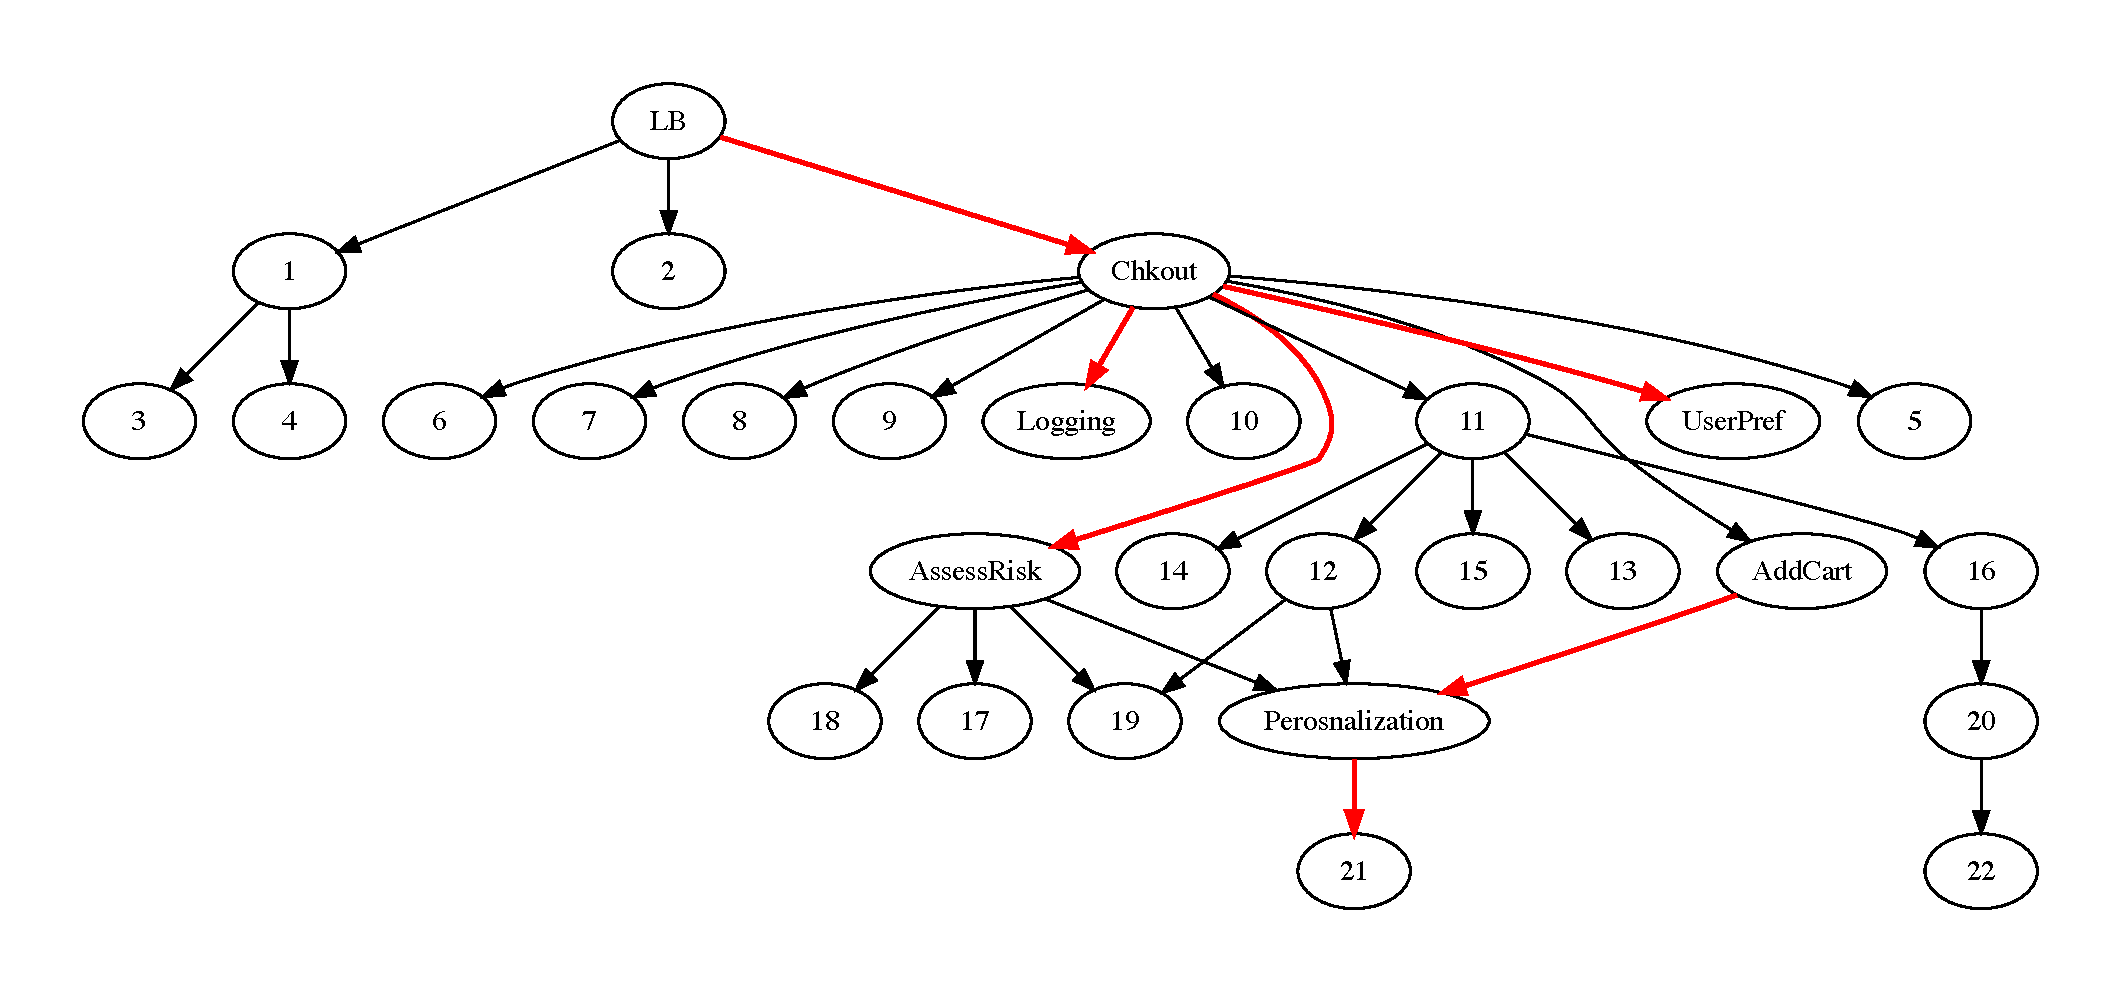
\includegraphics[scale=0.25]{anon_adrbk_fail.pdf}}
\caption{Example graph drawn from trace of a failed interaction. The red lines indicate that the callee has returned an error message to the caller}
\label{Failed_ex}
\end{figure}

To explain the triage process followed by site reliability engineers (SRE) when a failure occurs, we consider the example of a user trying to buy items from an online store. A successful checkout occurs when the user is able to place an order, else the checkout fails. Users being unable to checkout represents an outage of the system. Figure~\ref{Failed_ex} shows the  call-graph of a user interaction involving checkout of items for a cart during an outage. When users are unable to buy items form the store, it is the job of a site reliability engineer (SRE) to find out why. 
Currently, the SRE sees a number of alerts arising from failures, possibly in RPC calls highlighted as red in the call graph, from the monitoring system.  Subsequently, based on the alerts, the SRE may consult aggregate data such as error rates and latency over sliding windows of time for services deemed problematic.
The SRE might go about their job like so:
\begin{itemize}
\item Use domain knowledge about the dependencies between services to know which alerts are the result of transitive dependencies and must be ignored. \newline
As an example, the load balancer (LB) in the figure will be alerting as a result of its callee (Chkout) having returned an error message. This is indicated by the red line between LB and Chkout.  
An SRE with a good mental model of the system would conclude that since checkout (Chkout) has multiple downstream alerts, the alerts at LB are probably a result of the error being propagated up and try to dig deeper into one of the alerts from the downstream services. The reasoning is that a downstream service generating an alert is more likely to be a candidate for the proximal cause of the problem.  
\item Determine if the failure of some service(s) is the proximal cause \newline
Once a promising alert has been found, it is now time to look at the logs from the appropriate time to try to determine cause of failure. If the SRE determines service failure(s) to be proximal cause of the outage is caused by failure of mandatory services or a fallback path not being taken, she now has to \emph{obtain and compare} the trace of failed execution with that of one or more successful executions exercising the same request path. 
\end{itemize}

Both of the steps described above can be solved by comparing the trace of the failed execution with a family of successful traces in order to determine how the failed trace diverges from the successful traces. By witnessing a large number of successful executions during steady state, we can learn models from steady state data such that we construct representations for traces which encode the structural properties of the underlying graphs corresponding to the traces. Our technique for generating them derives from Word2Vec, which is used to generate word embeddings based on context of words in a sentence. Therefore, the trace representations learnt by our technique are called trace embeddings. Embeddings  serve two purposes:
\begin{enumerate}
\item Embeddings for traces can be classified before they are stored making it easy to find the most appropriate traces to compare to when a failure occurs.
\item As the number as well as the size of traces increase, storing the embeddings may be much more compact than the original traces. \kam{Since we haven't tried reversing our embedding to recapture the graphs, there may be some information loss here which we will need to quantify while making this claim. If we want to make this claim, that is}
\end{enumerate}

In the next section, we describe our technique for generation of trace embeddings and the corresponding distance measure used. In the evaluation, we describe how we use the fairly simple operations on the embeddings to address the problem described above and automatically generate hints about the proximal causes for the failure observed. 
%This is made possible by the fact that the embeddings encode information of structural neighborhoods.
%For outages which are not a result of service failures, a user entering invalid payment details perhaps or infrastructure failures, for example, appropriate next steps need to be taken. 

%-------------------------------------------------------------------------------
\section{Methodology}
%-------------------------------------------------------------------------------
Graph representation:  Aggregate of its component node (service) representations

Aggregator function: Summation

While there are other aggregator functions that we can use, summation is the simplest and has been used to obtain graph representations in previous work\kam{TODO: Needs citation}. The aggregate representation obtained can also be intuitively thought of as a linear combination of all the nodes present into the graph. 

Service representations : Obtained by using prior work, node2vec\kam{TODO citation}, which employs similar techniques as word2vec but for graphs. Graph nodes, in this case services, are analogous to words, and random walks in the graph generate for us sentences in the doc to train.


%-------------------------------------------------------------------------------
\section{Evaluation}
%-------------------------------------------------------------------------------
Sanity check: \newline
%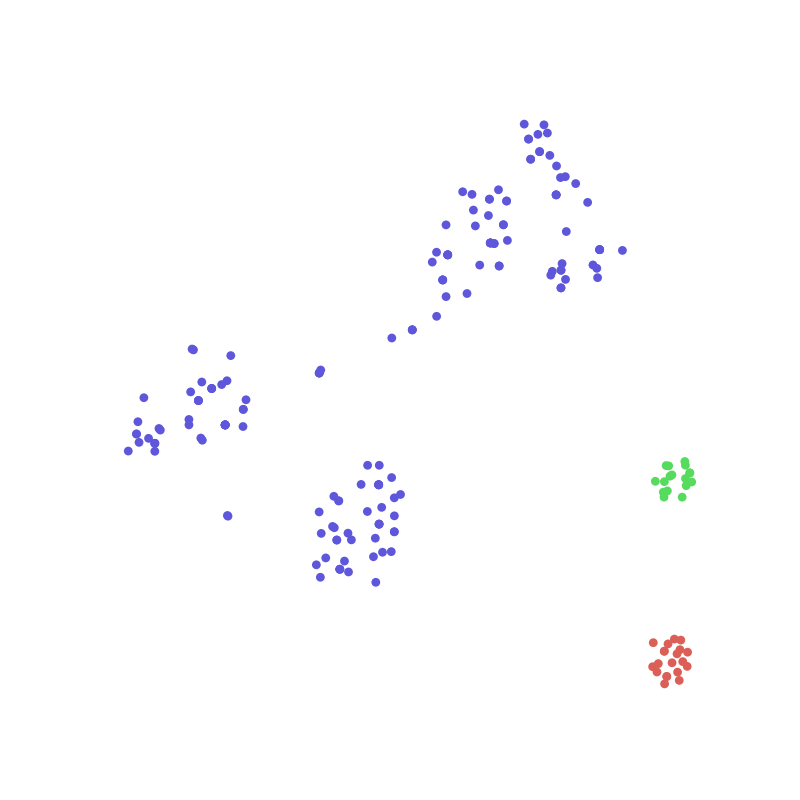
\includegraphics[scale=0.2]{tsne_viz.png}
\begin{itemize}
\item Classification: \newline 
Why classification? 
We are able to learn clusters accurately, but the problem is that using the clusters for predictive analysis performs poorly. The reason is that clusters are diffuse and in order to predict if a graph is in a cluster or not, the arithmetic mean of all pints in the cluster is computed. Doing so, however, results in information loss and leads to inaccurate results.

I started with a set of good graphs and a restricted set of test graphs
Classification worked perfectly when we have 16-dimensional vectors for the nodes \ newline
%\includegraphics[scale=0.4]{logistic_2d.png} \newline
%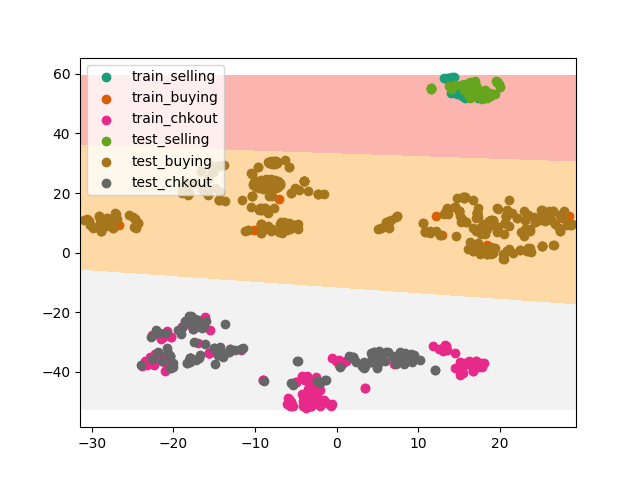
\includegraphics[scale=0.4]{test_logistic_2d.png} \newline

Q: Can we reduce the dimensions further?
When the dimensions were reduced to 4, a few graphs were mis-classified but not many  i.e. earlier there were no misclassification, now 1 in 575 graphs was misclassified

Take-away: Only small amount of information was required for classification, enabling compression

\item Predicting missing nodes and edges:  \newline
The way the problem is set up is that we have a graph that may be missing some nodes and/or edges. We have a set of complete graphs. Which one of them is the completion to our graph?
We can use euclidean distance between the representation for our graph and the target graph and choose the one that minimizes it. The traditional way to do this , however, is to use graph edit distance. 

Q: Do our results approximate computing the graph edit distance approach? 
To compute this, we implemented both approaches and then computed mean, median and mode for each of the two approaches. As the number of dimensions increased from 4 to 16, the gap between the two approaches narrowed. 

Q: Can we eliminate this gap? What if we choose number of dimensions to be 128?
Turns out 128 dimensions is only a slight improvement over 16

Take away: This question requires more information to be retained as compared with classification.
\end{itemize}



%-------------------------------------------------------------------------------
\section{Related Work}
%-------------------------------------------------------------------------------

\ash{
Post factum analysis of traces is important because they contain useful information like causality of events, resource consumption, errors, performance data and labeled metdata about components involved in the execution.
In large systems the size of the traces makes it impractical for a developer to do any manual analysis. This motivates the need for automated analysis of large corpus of traces to derive useful insights.
There are many goals for analysis for traces, including finding performance bottlenecks, system recovery \& repair, debugging, resource usage, service degradation analysis.
Many of these use cases use some form of classification or clustering. We descrobe some of the prior work in this area and highlight the drawbacks and explain how our approach overcomes some of the hurdles.
}

\ash{
Magpie \cite{Barham:2003:MOM:1251054.1251069} relies on structured events produced logged by ETW (event tracing for windows) inorder to avoid the need to have unique identifiers for every request.
Magpie correlates events generated by the application, middleware and operating system using temporal joins to infer causal relationships. 
Magpie uses a comparison based on a simple string-edit-distance metric on flattened execution graphs as a basis for execution clustering.
Even though the technique shows promising results even for classification of requests with differences in internal concurrency structures, the authors acknowledge the need for graph and tree edit distances.
}

\ash{
Pinpoint \cite{Chen:2004:PFE:1251175.1251198} collects execution traces as a series of paths through the system. The authors diagnose anomalies by generating a probabilistic context-free grammar (PCFG) from the paths. 
They perform anomaly detection at runtime, whereby new paths are compared to the generated model to determine the probability with which it would be produced from the grammar. 
Anomaly detection worked well in experiments, but the authors note that there are a number of realistic scenarios where it would
not work well: features must be represented in the training set for them to be considered at runtime; changes
such as software upgrade require the model to be retrained;and the learned model represents a superset of observed paths.
}

\ash{
Spectroscope \cite{Sambasivan:2011:DPC:1972457.1972463} collects execution traces represented as process invocation trees, and diagnoses performance
changes by comparing sets of before- and aftertraces. Spectroscope assumes that a similar workload was run before and after the performance change, and that the performance change manifests as a change in distribution
over the request structures and/or request timings. To diagnose a change, spectroscope compares the distributions of service completion times for graphs that are topologically identical, and compares structural differences
between executions using string-edit-distance.
}

\ash{
Mann et al. \cite{Mann:2011:MPE:2170444.2170464} collect execution traces from datacenter services, and model the latency of a service given the child services invoked.
This work focuses on learning join-point locations by comparing large volumes of Dapper traces.
The execution graphs recorded do not fully capture the causal dependencies internal to a service, so one component of the work is to deduce those causal dependencies from a collection of training examples.
The training examples are then clustered if they have identical execution graphs. 
At runtime, a cluster is selected by comparing its service timings with the cluster centroids, and selecting the nearest-neighbour. 
A prediction for the execution’s overall runtime is then given based on the other executions in the selected cluster.
}

\ash{
Mann et al. and Spectroscope do clustering, but only for graphs that are isomorphic. 
For graphs with different topology, Spectroscope and Magpie use string-editdistance on canonicalized and linearized graphs as a metric,
for proper clustering in the latter, and for finding similar clusters in the former.
Magpie and Pinpoint cluster similar behavior and suggest outliers as possible indicators of bugs.
}

\ash{
Pip \cite{Reynolds2006PipDT} takes a different approach to solving these problems. 
Unlike Magpie Pip does not rely on any statistical inference and hence obviates the need to collect a large corpus of traces.
Pip treats the systems as \textit{grey-box} and finds structural and performance bugs in distributed systems by comparing actual system behavior to expected system behavior.
Pip asks the developers to specify the expectations of the program using a declarative specification language, while capturing the actual system behavior using instrumentation, annotations or sniffing.
Pip automatically checks actual behavior against expected behavior and helps programmers visualize the result to discover the causes of any unexpected behavior.
However, pip cannot be used for analysis of running programs since it waits for the program to terminate before reconciling traces. 
This makes pip unsuitable for use in online services. 
}

%-------------------------------------------------------------------------------
\section{Conclusions and Future Work}
%-------------------------------------------------------------------------------
\begin{itemize}
\item Representations:
    \begin{enumerate}
    \item Use a different aggregator function other than sum:
    This will probably be necessary for synthetic trace generation. Currently, we cannot convert a representation into a trace. 
    \item Assign weights to services based on their importance.
    \item Use tranductive models to get representations for services not seen in training.
    \end{enumerate}
\item Fault diagnosis
    \begin{enumerate}
    \item We are curating our corpus to add more failed graphs. Want to show examples suggesting a successful trace in which a fallback path was taken as a potential hint.
    \item We need to remember some corpus of successful graphs to compare against. The next step would be to learn a few canonical graphs representing successful executions that we can use when providing hints.
    \end{enumerate}
\item Response time mutations
For fault diagnostics, we only considered cases when the unsuccessful execution was not calling out to some expected services. There are failures in which the only differential is response time. For such failure cases, might incorporating latency into representations be a good idea?
\item Other technqiues
    \begin{enumerate}
    \item Graph convolutional networks and autoencoders may be other techniques that may be applicable in this context
    \item Comparisons of these via-a-vis our current technique might be useful to highlight strengths and weaknesses of each.
    \end{enumerate}
\end{itemize}




%-------------------------------------------------------------------------------
%\section*{Acknowledgments}
%-------------------------------------------------------------------------------

%-------------------------------------------------------------------------------
\bibliographystyle{plain}
\bibliography{references}

%%%%%%%%%%%%%%%%%%%%%%%%%%%%%%%%%%%%%%%%%%%%%%%%%%%%%%%%%%%%%%%%%%%%%%%%%%%%%%%%
\end{document}
%%%%%%%%%%%%%%%%%%%%%%%%%%%%%%%%%%%%%%%%%%%%%%%%%%%%%%%%%%%%%%%%%%%%%%%%%%%%%%%%

%%  LocalWords:  endnotes includegraphics fread ptr nobj noindent
%%  LocalWords:  pdflatex acks
